
%(BEGIN_QUESTION)
% Copyright 2011, Tony R. Kuphaldt, released under the Creative Commons Attribution License (v 1.0)
% This means you may do almost anything with this work of mine, so long as you give me proper credit

Calculate the volume of liquid stored inside this vessel when the measured liquid height within the vessel is 4.5 feet, assuming the vessel's shape is a vertical cylinder with a 7.4 foot diameter:

$$\includegraphics[width=15.5cm]{i03450x01.eps}$$

$V$ = \underbar{\hskip 50pt} cubic feet

\vskip 10pt

Also, write a single equation solving for stored liquid volume ($V$) in terms of height ($h$) and diameter ($d$). 

\underbar{file i03450}
%(END_QUESTION)





%(BEGIN_ANSWER)

$V$ = \underbar{\bf 193.54} cubic feet \hskip 30pt $V = {{\pi d^2 h} \over 4}$

\vskip 10pt

5 points for numerical answer, 5 points for equation.

%(END_ANSWER)





%(BEGIN_NOTES)

{\bf This question is intended for exams only and not worksheets!}.

%(END_NOTES)


